\section[C. simétrico en la práctica]{Cifrado simétrico en la práctica}
\subsection{Redes de sustitución y permutación}
Las redes de sustitución y permutación (SP-networks) son una estructura común utilizada en muchos algoritmos de cifrado por bloques, incluido AES, que profundizaremos un poco más adelante. Consisten en una serie de rondas de sustitución (S) y permutación (P), que juntas proporcionan una mezcla fuerte de los bits de entrada.

\begin{itemize}
    \item \textbf{Sustitución (S):} En esta etapa, los bloques de bits de entrada se transforman mediante una operación no lineal. En el caso de AES, esto se realiza en la etapa SubBytes, donde cada byte del estado se sustituye por otro byte según una tabla de sustitución predefinida llamada S-box. Esta tabla ha sido diseñada para ser resistente a varios tipos de ataques criptográficos, y proporciona la propiedad de \textbf{confusión} en el cifrado, lo que significa que los bits de salida deben depender de manera compleja y no lineal de los bits de la clave.
    
    \item \textbf{Permutación (P)}: Después de la sustitución, los bits se reorganizan (o se permutan). Esto esencialmente dispersa las correlaciones estadísticas introducidas por la etapa de sustitución. En AES, esto se realiza en las etapas ShiftRows y MixColumns. ShiftRows es una operación de permutación simple que reordena los bytes dentro de cada bloque. MixColumns es una operación de permutación más compleja que mezcla los bytes entre los bloques. Estas operaciones proporcionan la propiedad de \textbf{difusión} en el cifrado, lo que significa que si un solo bit de entrada cambia, entonces los bits de salida deberían cambiar de manera aparentemente aleatoria e impredecible.
\end{itemize}
\fig{img/cap4/1.png}{0.325}{Representación de las sustituciones y permutaciones}

Las SP-networks son poderosas porque combinan la confusión (alterando los valores de los datos) y la difusión (alterando la ubicación de los datos). Estas dos propiedades juntas hacen que el cifrado sea muy difícil de romper sin conocer la clave, porque cualquier cambio pequeño en la clave o en el texto plano de entrada debería producir cambios grandes y aparentemente aleatorios en el texto cifrado de salida. \bigbreak

El diseño de la S-box y las operaciones de permutación en AES tiene una base sólida en la teoría de números y la aritmética de campos finitos. Esta base teórica es una de las razones por las que AES es considerado seguro contra muchos tipos de ataques criptográficos.

\newpage

\subsection{Advanced Encryption Standard (AES)}
AES es un algoritmo de cifrado por bloques que fue establecido por el Instituto Nacional de Estándares y Tecnología (NIST) de los Estados Unidos en 2001. Es un algoritmo de cifrado simétrico, lo que significa que utiliza la misma clave para cifrar y descifrar los datos. Esta clave puede tener una longitud de 128, 192 o 256 bits, lo que da lugar a las variantes AES-128, AES-192 y AES-256, respectivamente. \medbreak

AES opera en bloques de datos de 128 bits, independientemente de la longitud de la clave. Si los datos que se van a cifrar no son múltiplos de 128 bits, deben rellenarse hasta el tamaño correcto. Además, AES es una \textbf{red de sustitución}, con 10 rondas para AES-128, 12 rondas para AES-192 y 14 rondas para AES-256. \medbreak

Durante el cálculo del algoritmo AES, una matriz de 4x4 bytes llamada \textbf{matriz de estado} se modifica en una serie de rondas. La matriz de estado se establece inicialmente igual a la entrada del cifrado (notar que la entrada es de 128 bits, que son exactamente 16 bytes). 
\fig{img/cap4/2.png}{0.4}{Matriz de estado}

Estudiemos el caso de AES-128. En cada ronda, las siguientes operaciones se aplican a la matriz de estado:

\begin{enumerate}
    \item \textbf{AddRoundKey:} Se deriva, desde el \textit{key schedule}, una subllave de 128 bits de la llave principal y se ve como una matriz de 4x4 bytes. La matriz de estado se actualiza mediante un XOR con esta nueva llave.
    \fig{img/cap4/6.png}{0.3}{Representación de la matriz de una llave}

    El \textit{key schedule} que genera las subllaves de todas las rondas funciona, a grandes rangos, de la siguienta manera:
    \begin{itemize}
        \item A la última columna de la matriz de 4x4 de la llave principal se realiza una operación \textbf{RotWord} que rota el primer byte de la columna al final de la misma.
        \fig{img/cap4/7.png}{0.3}{Representación de RotWord}

        \item Se realiza una operación \textbf{SubWord} en el resultado de la operación RotWord. Esta operación aplica la $S$-box de AES a cada byte de la palabra clave.
        \fig{img/cap4/8.png}{0.3}{Representación de RotWord}
        
        \item Se realiza una operación XOR entre el resultado de Subword, la columna que está 3 posiciones detrás (la primera columna de la llave principal), y una columna que es única por cada llave por ronda denominada \textbf{Rcon}.
        \fig{img/cap4/9.png}{0.3}{Representación de Rcon}

        \item La primera iteración de RotWord, SubWord y Rcon dan origen a la primera columna de la primera subllave, para luego seguir con el proceso de hacer XOR con la columna 3 posiciones detrás hasta obtener las 4 columnas de la primera subllave.
        
        \begin{itemize}
            \item La primera columna de la subllave hace XOR con la segunda de la llave principal, obteniendo la segunda columna de la subllave.
            \item La segunda columna de la subllave hace XOR con la tercera de la llave principal, obteniendo la tercera columna de la subllave.
            \item Finalmente, la tercera columna de la subllave hace XOR con la cuarta (última) columna de la llave principal, obteniendo la cuarta columna de la subllave, y completando así la matriz.
        \end{itemize}
        
        \item Este proceso se repite hasta obtener las 10 subllaves para cada ronda, recordando que Rcon es un vector único en cada una de las rondas.
    \end{itemize}
    
    \item \textbf{SubBytes:} En este paso, cada byte de la matriz de estado se reemplaza por otro byte de acuerdo a una única tabla de búsqueda fija $S$. Esta tabla de sustitución (o $S$-box) es una permutación en $\{0,1\}^8$.
    \fig{img/cap4/3.png}{0.4}{Representación de SubBytes}
    
    \item \textbf{ShiftRows:}  A continuación, los bytes en cada fila de la matriz de estado se mezclan de la siguiente manera: la primera fila de la matriz no se toca, cada byte de la segunda fila se desplaza un lugar a la izquierda, la tercera fila se desplaza dos lugares a la izquierda, y la cuarta fila se desplaza tres lugares a la izquierda.
    \fig{img/cap4/5.png}{0.4}{Representación de ShiftRows}
    
    \item \textbf{MixColumns:} Finalmente, se aplica una transformación lineal invertible a los cuatro bytes en cada columna. Esta transformación tiene la propiedad de que si dos entradas difieren en $b > 0$ bytes, entonces las salidas resultantes difieren en al menos $5 - b$ bytes.
    \fig{img/cap4/10.png}{0.4}{Representación de MixColumns}
\end{enumerate}

En la última ronda, MixColumns se reemplaza con AddRoundKey. Esto evita que un adversario simplemente invierta las últimas tres etapas, que no dependen de la clave. \medbreak
\begin{figure}[H]
    \centering
    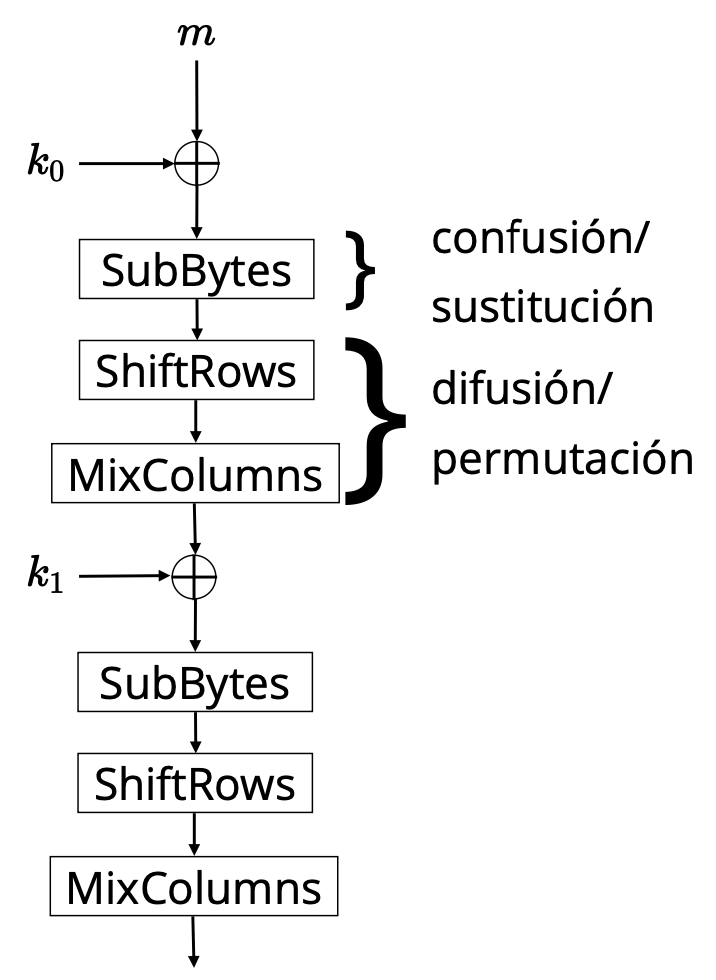
\includegraphics[scale=0.4]{img/cap4/11.png}
    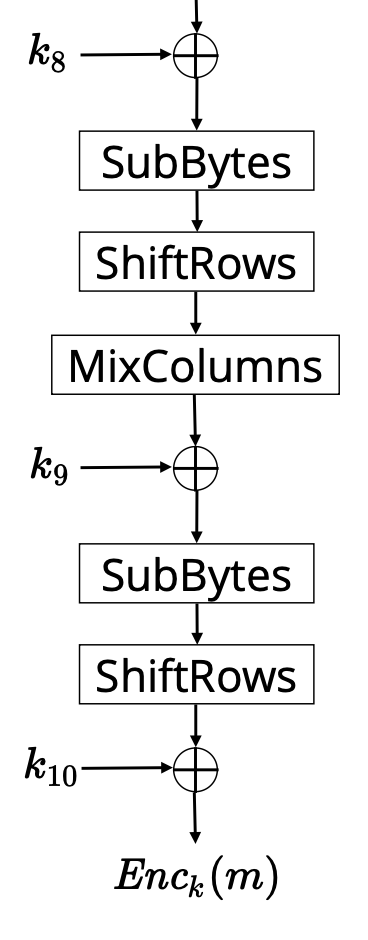
\includegraphics[scale=0.4]{img/cap4/12.png}
    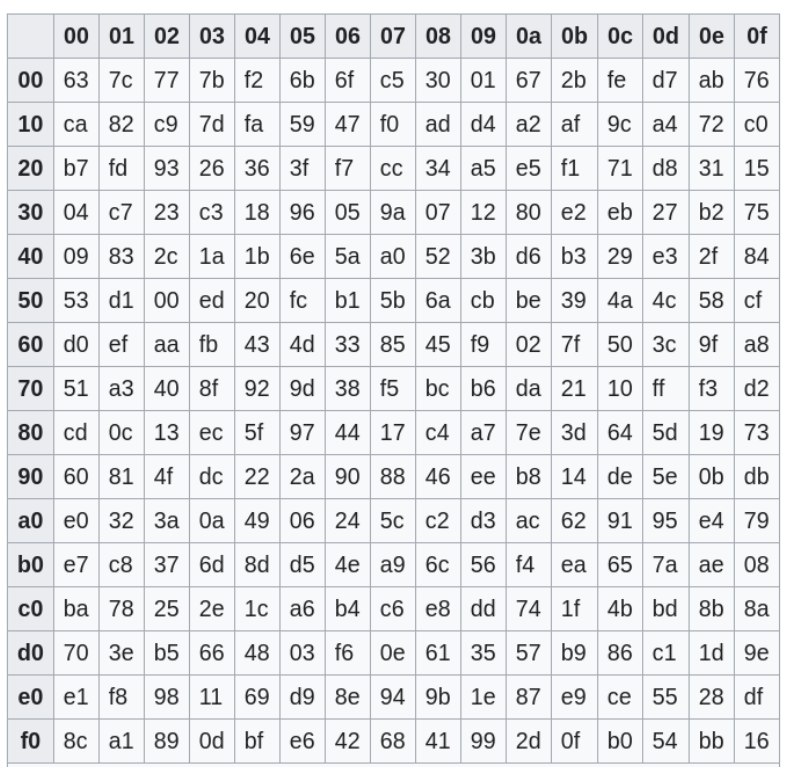
\includegraphics[scale=0.5]{img/cap4/4.png}
    \caption{Ejemplo de AES-128 y la $S$-box}
\end{figure}
